\documentclass[conference]{IEEEtran}
\IEEEoverridecommandlockouts
% The preceding line is only needed to identify funding in the first footnote. If that is unneeded, please comment it out.

% RULES: 
% The length for final papers is a maximum of 4-6 pages without exceptions.
% Each paper should indicate appropriateness for the conference's scope, originality, quality of the technical content, whole organization, and writing style. The paper should, moreover, explain the significance of the contribution and contain a list of key references.
% A submission implies a willingness to register and present the work if the paper is accepted for presentation at the Conference.
\usepackage{cite}
\usepackage{amsmath,amssymb,amsfonts}
\usepackage{algorithmic}
\usepackage{graphicx}
\usepackage{textcomp}
\usepackage{subcaption}
\usepackage{xcolor}
\usepackage{hyperref}
\usepackage{cleveref}
\def\BibTeX{{\rm B\kern-.05em{\sc i\kern-.025em b}\kern-.08em
    T\kern-.1667em\lower.7ex\hbox{E}\kern-.125emX}}
\begin{document}

\title{Automated Passive Tracking for MR-guided Endovascular Interventions}

\author{\IEEEauthorblockN{Martin Reinok}
\IEEEauthorblockA{\textit{Robotics and Mechatronics Group,}\\
\textit{Faculty of EEMCS} \\
\textit{University of Twente}\\
Enschede, Netherlands \\
m.reinok@student.utwente.nl}
\and
\IEEEauthorblockN{Giulio Dagnino}
\IEEEauthorblockA{\textit{Robotics and Mechatronics Group,}\\
\textit{Faculty of EEMCS} \\
\textit{University of Twente}\\
Enschede, Netherlands \\
g.dagnino@utwente.nl}
\and
\IEEEauthorblockN{Wyger Brink}
\IEEEauthorblockA{\textit{Magnetic Detection and Imaging Group,}\\
\textit{Technical Medical Centre} \\
\textit{University of Twente}\\
Enschede, Netherlands \\
w.m.brink@utwente.nl}
}

\maketitle

\begin{abstract}
Vascular and cardiac interventions often rely on X-ray fluoroscopy for real-time imaging guidance, which poses risks due to ionizing radiation exposure. MRI offers a safer alternative with superior soft tissue contrast and avoids using ionizing radiation, but its adoption for near real-time guidance so far has been limited by technical challenges. This paper presents a novel approach for real-time detection and tracking of an MR-visible guidewire with discrete markers during endovascular interventions, addressing key limitations. A series of experiments was designed to evaluate and
optimize marker visibility in terms of contrast-and-noise for different sequences. A convolutional neural network (CNN) is trained to detect the marker artefacts using a physics-based marker model and evaluated experimentally in an aortic phantom. The physics-based model simulation is used to generate the dataset without the need for MRI imaging, or manually annotating dataset for training the CNN model. The output from the CNN model is integrated into a custom software interface that links the tracked markers to automatic MRI slice geometry alignment, enabling near real-time guidewire tracking. Experimental results evaluate the effectiveness of the proposed approach in detecting the guidewire under varying imaging conditions, showing promise in improving the safety, efficiency, and accuracy of MR-guided interventions.
\end{abstract}

\begin{IEEEkeywords}
MRI-guided interventions, passive tracking, susceptibility artefacts, endovascular interventions
\end{IEEEkeywords}

\section{Introduction}
Cardiovascular diseases continue to be the leading cause of death in the world, representing 32 \% of the global deaths \cite{webcardio}. Image-guided endovascular intervention forms the current clinical standard in treatment, with a reduced risk of complications and shorter recovery time compared to open surgery \cite{Jung2018}. While X-ray fluoroscopy is currently the preferred modality for real-time imaging due to its commendable spatial and temporal resolution, it has notable drawbacks including limited soft tissue characterization and exposure to ionizing radiation for patients and medical staff. As an alternative to fluoroscopy, MRI provides excellent soft-tissue contrast, is capable of imaging in an arbitrary slice orientation and completely free of ionizing radiation. Both clinical and experimental studies conducted using MRI have demonstrated its potential in various interventional procedures, including the delivery of Atrial Septal Defect (ASD) closure, placement of aortic valves and endovascular stents \cite{pmid21359519}.

Despite these benefits, MRI has a number of drawbacks that limit its application during interventional procedures. These include the relatively low spatio-temporal resolution, difficulties in device visibility, intermittent manual slice alignment hampering the procedure, as well as safety considerations related to device heating \cite{pmid35420239}. MRI in general involves a trade-off between spatial resolution, signal-to-noise ratio (SNR) and acquisition time. Even though the spatial resolution can potentially compare to that of X-ray fluoroscopy, the associated acquisition time makes that real-time capabilities drop significantly \cite{Green2005}. Introduction of a sliding window technique allowed initial implementations to already reach frame rates of up to 30 Hz which is close to on-par with fluoroscopy, albeit at the cost of image quality \cite{pmid3173063}. %In most interventional procedures, an imaging frame rate of 2-3 Hz may also be considered acceptable compromise between spatial/temporal resolution. 

In terms of device visibility either active and passive tracking can be considered for MR-guided endovascular procedures. Active tracking involves integrating a miniaturized RF receive coil and associated electronics into the device, producing a strong localized receive intensity that can be localized very efficiently using dedicated tracking sequences \cite{pmid11146480}. Passive  tracking, on  the  other  hand, is based on embedding a small magnetic susceptibility marker into the device, such as iron oxides or stainless steel, which produces a localized static magnetic field distortion and associated susceptibility artefact when imaged. \autoref{fig:xray-vs-mri-guidewire-comparison} compares the visibility of a guidewire under fluoroscopy and MRI. Although the conspicuity of this artefact depends on MRI acquisition settings, an adequate spatial-temporal resolution can generally be achieved by using fast gradient-echo based sequences \cite{pmid11146480}. Devices suited for passive tracking may be less costly to produce and involve fewer safety concerns as there are no electrical interconnections required to the MR system. Downsides include potential out-of-plane motion and manual readjustment of the acquisition settings by the external operator, which hampers the interventional procedure.
% \textbf{TODO: What has been done in literature to fix these problems}

\begin{figure}[h]
    \centering
    \begin{minipage}{0.241\textwidth}
        \centering
        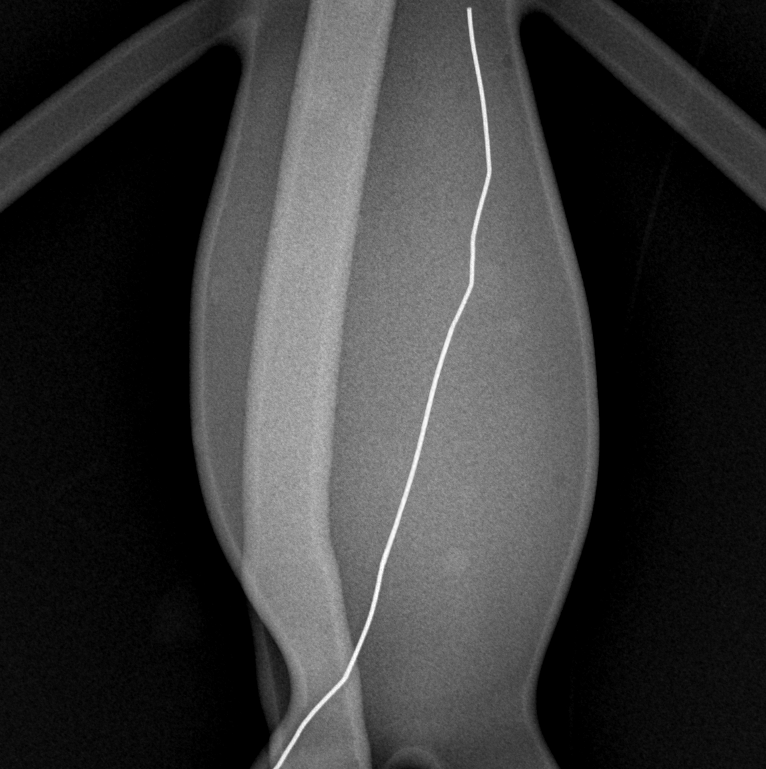
\includegraphics[width=\textwidth]{Conference/img/xray-device-visibility.png}
        \subcaption*{(a)}
    \end{minipage}\hfill \hspace*{0cm}
    \begin{minipage}{0.241\textwidth}
        \centering
        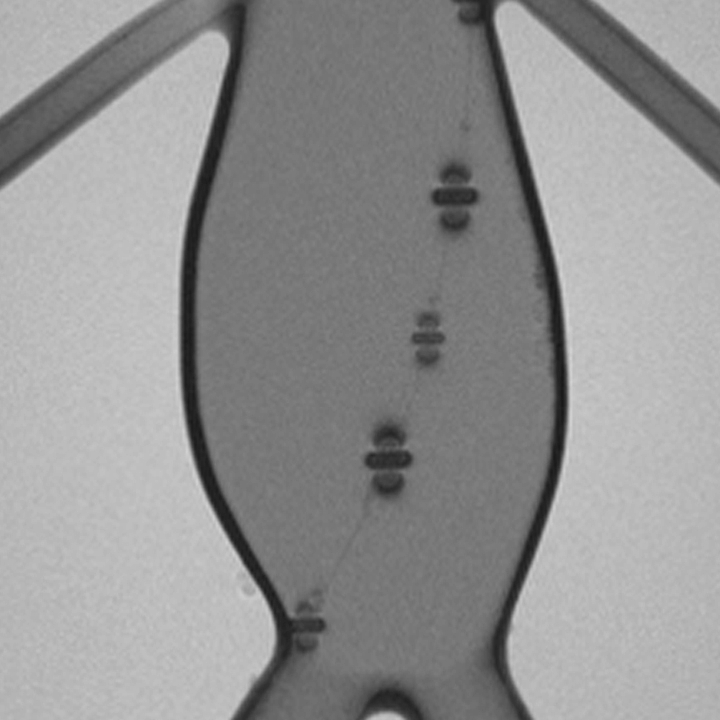
\includegraphics[width=\textwidth]{Conference/img/mri-device-visibility.jpg}
        \subcaption*{(b)}
    \end{minipage}\hfill \hspace*{0cm}
    \caption{Coronal images of silicone phantom comparing endovascular device visibility under (a) X-ray fluoroscopy and (b) MRI.}
    \label{fig:xray-vs-mri-guidewire-comparison}
\end{figure}

In this study, we evaluate a novel automated approach to passive tracking which involves detecting the passive markers carried by an endovascular guidewire from a real-time MR image datastream and adjusting the slice geometry accordingly. Robust detection is achieved efficiently using a physics-informed CNN, which avoids extensive manual annotation of training data. After detection, dynamic behaviour of the markers is identified followed by automatic slice alignment to track the guidewire. The proposed approach aims to provide a comprehensive and cost-effective solution for MR-guided interventions.
% \textbf{TODO: What we propose and how does it help}

\section{Methods}

\subsection{MRI system and protocol}\label{MRI-settings}

% any idea on the molarity of the MnCl2 solution?
% It was 0.018g MnCl2, 2000ml h2o (distilled)
All MR data was acquired on a 1.5T MRI system (\text{MAGNETOM} Aera, Siemens Healthineers, Erlangen, Germany) using an 18-channel torso RF coil and a 24-channel spine RF coil. An abdominal aortic aneurysm phantom made from silicone was modified to enable guidewire access \cite{pmid28689483} and the lumen compartment was filled with a 72 $\mu$M MnCl$_2$ blood-mimicking solution ($T_1 = 770$ ms and $T_2 = 200$ ms) while the outer compartment was filled with tapwater. The study is guided by an MR-visible guidewire which incorporates discrete passive markers (MRLine, EPflex, Dettingen an der Erms, Germany), resulting in local image artefacts as shown in \autoref{fig:xray-vs-mri-guidewire-comparison} (b).

A series of experiments was designed to evaluate and optimize marker visibility. Following earlier studies \cite{pmid3173063}, \cite{pmid16683261} we have evaluated both two-dimensional (2D) gradient-recalled-echo (GRE) and balanced steady-state free precession (bSSFP) sequences for a series of slice thicknesses. Apart from the parameters that affect mainly the spatial-temporal resolution of the sequence, such as number of phase encoding steps and time-of-repetition (TR), the slice thickness affects both the image SNR as well as conspicuity of the marker artefact and robustness with respect to out-of-place movement. A higher slice thickness may improve SNR but reduce the marker contrast due to partial volume effects. A thinner slice, on the other hand, can improve the marker contrast but may complicate the tracking performance due to out-of-plane movement of the markers. A suitable trade-off will help improve tracking performance.

The sequence parameters used in the optimization are listed in \autoref{table_MRI_parameters}. The starting point for the optimization was to acquire a field-of-view (FOV) of 350 mm within approximately 500 ms to enable smooth procedural imaging. The slice thickness was varied from 2.5 up to 30 mm to compare its influence on marker contrast-to-noise ratio (CNR), defined as the difference in mean signal at the marker location with respect to the surrounding lumen, divided by the standard deviation of background noise. Finally, for both sequences a minimum time-of-repetition (TR) and echo-time (TE) was enforced to minimize scan time and maximize the attainable in-plane spatial resolution.

\begin{table}[ht]
\centering
\caption{MR sequence optimization}
\label{table_MRI_parameters}
\begin{tabular}{|l|l|l|}
    \hline & GRE & bSSFP \\
    \hline FOV & 350 & 350 \\
    \hline in-plane resolution [mm] & 1.4  & 1.4 \\
    \hline slice thickness [mm] & 2.5 - 30 & 2.5 - 30 \\
    \hline TR [ms] & 674  & 484 - 471 \\
    \hline TE [ms] & 1.99 & 1.49 \\
    \hline tip angle [\textdegree] & 15 & 50  \\
    \hline
\end{tabular}
\end{table}

\subsection{Susceptibility artefact model}\label{artefact-simulation}

The paramagnetic markers embedded on the guidewire create small local magnetic field distortions, which can be mathematically described as a magnetic dipole, as given by \cite{pmid14523965}:

\begin{equation}
\label{eq:dipole-field-distortion}
B_z = \frac{B_0 \cdot \Delta{\chi} V}{4 \pi} \cdot \frac{(x^2 + y^2 - 2z^2)}{(x^2 + y^2 + z^2)^{\frac{5}{2}}}
\end{equation}

Here, $B_0$ is the main magnetic field, $\Delta{\chi}$ is the susceptibility difference between the marker material and the surrounding tissues, $V$ is the volume of the paramagnetic material and $x$, $y$ and $z$ represent the spatial coordinates.

An example simulation of \eqref{eq:dipole-field-distortion} is shown in \autoref{fig:simulations}(a). To transform this magnetic field distortion into the image artefact in a coronal magnitude image, integration over the slice thickness is necessary \cite{pmid14523965}:

\begin{equation}
\label{eq:integration-over-slice-formula}
S_{coronal} = \int_{-d/2}^{d/2} {\rho}(x,y,z) \exp(-i\gamma B_z TE) \,dz
\end{equation}

Here, $\rho (x,y,z)$ is the spin density, $d$ is the slice thickness, $\gamma$ (Hz/T) is gyromagnetic ratio ($^1\text{H}$) and $TE$ the echo time. Simulation of \eqref{eq:integration-over-slice-formula} results in \autoref{fig:simulations}(b).

% the dipole field distortion looks phase-wrapped, the B0 field distortion should be consistently increasing as you get closer to the dipole center. Please check
\begin{figure}[h]
    \centering
    \begin{minipage}{0.241\textwidth}
        \centering
        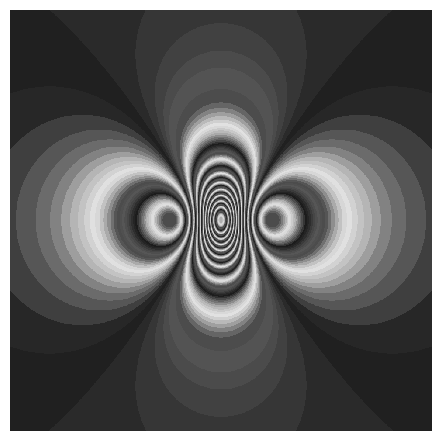
\includegraphics[width=\textwidth, angle=90]{Conference/img/dipole-field-distortion.png}
        \subcaption*{(a)}
    \end{minipage}\hfill \hspace*{0cm}
    \begin{minipage}{0.241\textwidth}
        \centering
        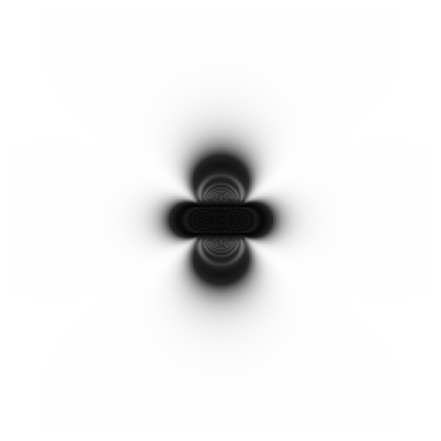
\includegraphics[width=\textwidth]{Conference/img/coronal-magnitude-simulation.png}
        \subcaption*{(b)}
    \end{minipage}\hfill \hspace*{0cm}
    \caption{(a) Example dipole field distortion,
    (b) simulated coronal magnitude.}
    \label{fig:simulations}
\end{figure}

\subsection{CNN-based marker detection}\label{training-cnn}

For training the CNN to detect susceptibility artefacts, we utilized a nnUNet framework which provides a robust infrastructure for medical image segmentation tasks \cite{pmid33288961}. The training process was conducted using the following specifications (configured automatically by nnUNet):
\begin{itemize}
    \item \textbf{Features}: 32.
    \item \textbf{Convolutions}: 2, for both encoder and decoder.
    \item \textbf{Kernel Sizes}: Pooling: $2 \times 2$, and convolutional layers: $3 \times 3$.
    \item \textbf{Image size}: (upsampled) $512 \times 512$ pixels
\end{itemize}

\subsection{Physics-based dataset augmentation}\label{artefact-cnn-dataset}

To increase the diversity of training data and avoid time-consuming manual annotation of susceptibility artefacts, an alternative physics-based approach is presented. The generated susceptibility artefact is first masked by it's signal value, resulting in a ground truth mask. The generated artefact is then superimposed on existing MRI images by means of pixel-wise multiplication. The size, contrast and the number of artefacts on the image are augmented within a suitable range, reflecting realistic variations in data.

A dataset of 26 background images was used, which included phantom MR images, in-vivo cardiac MR images from an online database \cite{pmid29994302} and plain background images with variable noise and resolution, examples shown in \autoref{fig:background-dataset}. A region of interest was chosen for each image, to limit the placement range of artefacts. In order to avoid overlapping marker artefacts, the placement of additional artefacts was further restricted to satisfy a minimum distance in between markers. An example of the generated image, with corresponding ground truth mask is shown in \autoref{fig:generated-dataset-and-truth}.

% \textbf{TODO: MRI sequence settings!}

\begin{figure}
    \centering
    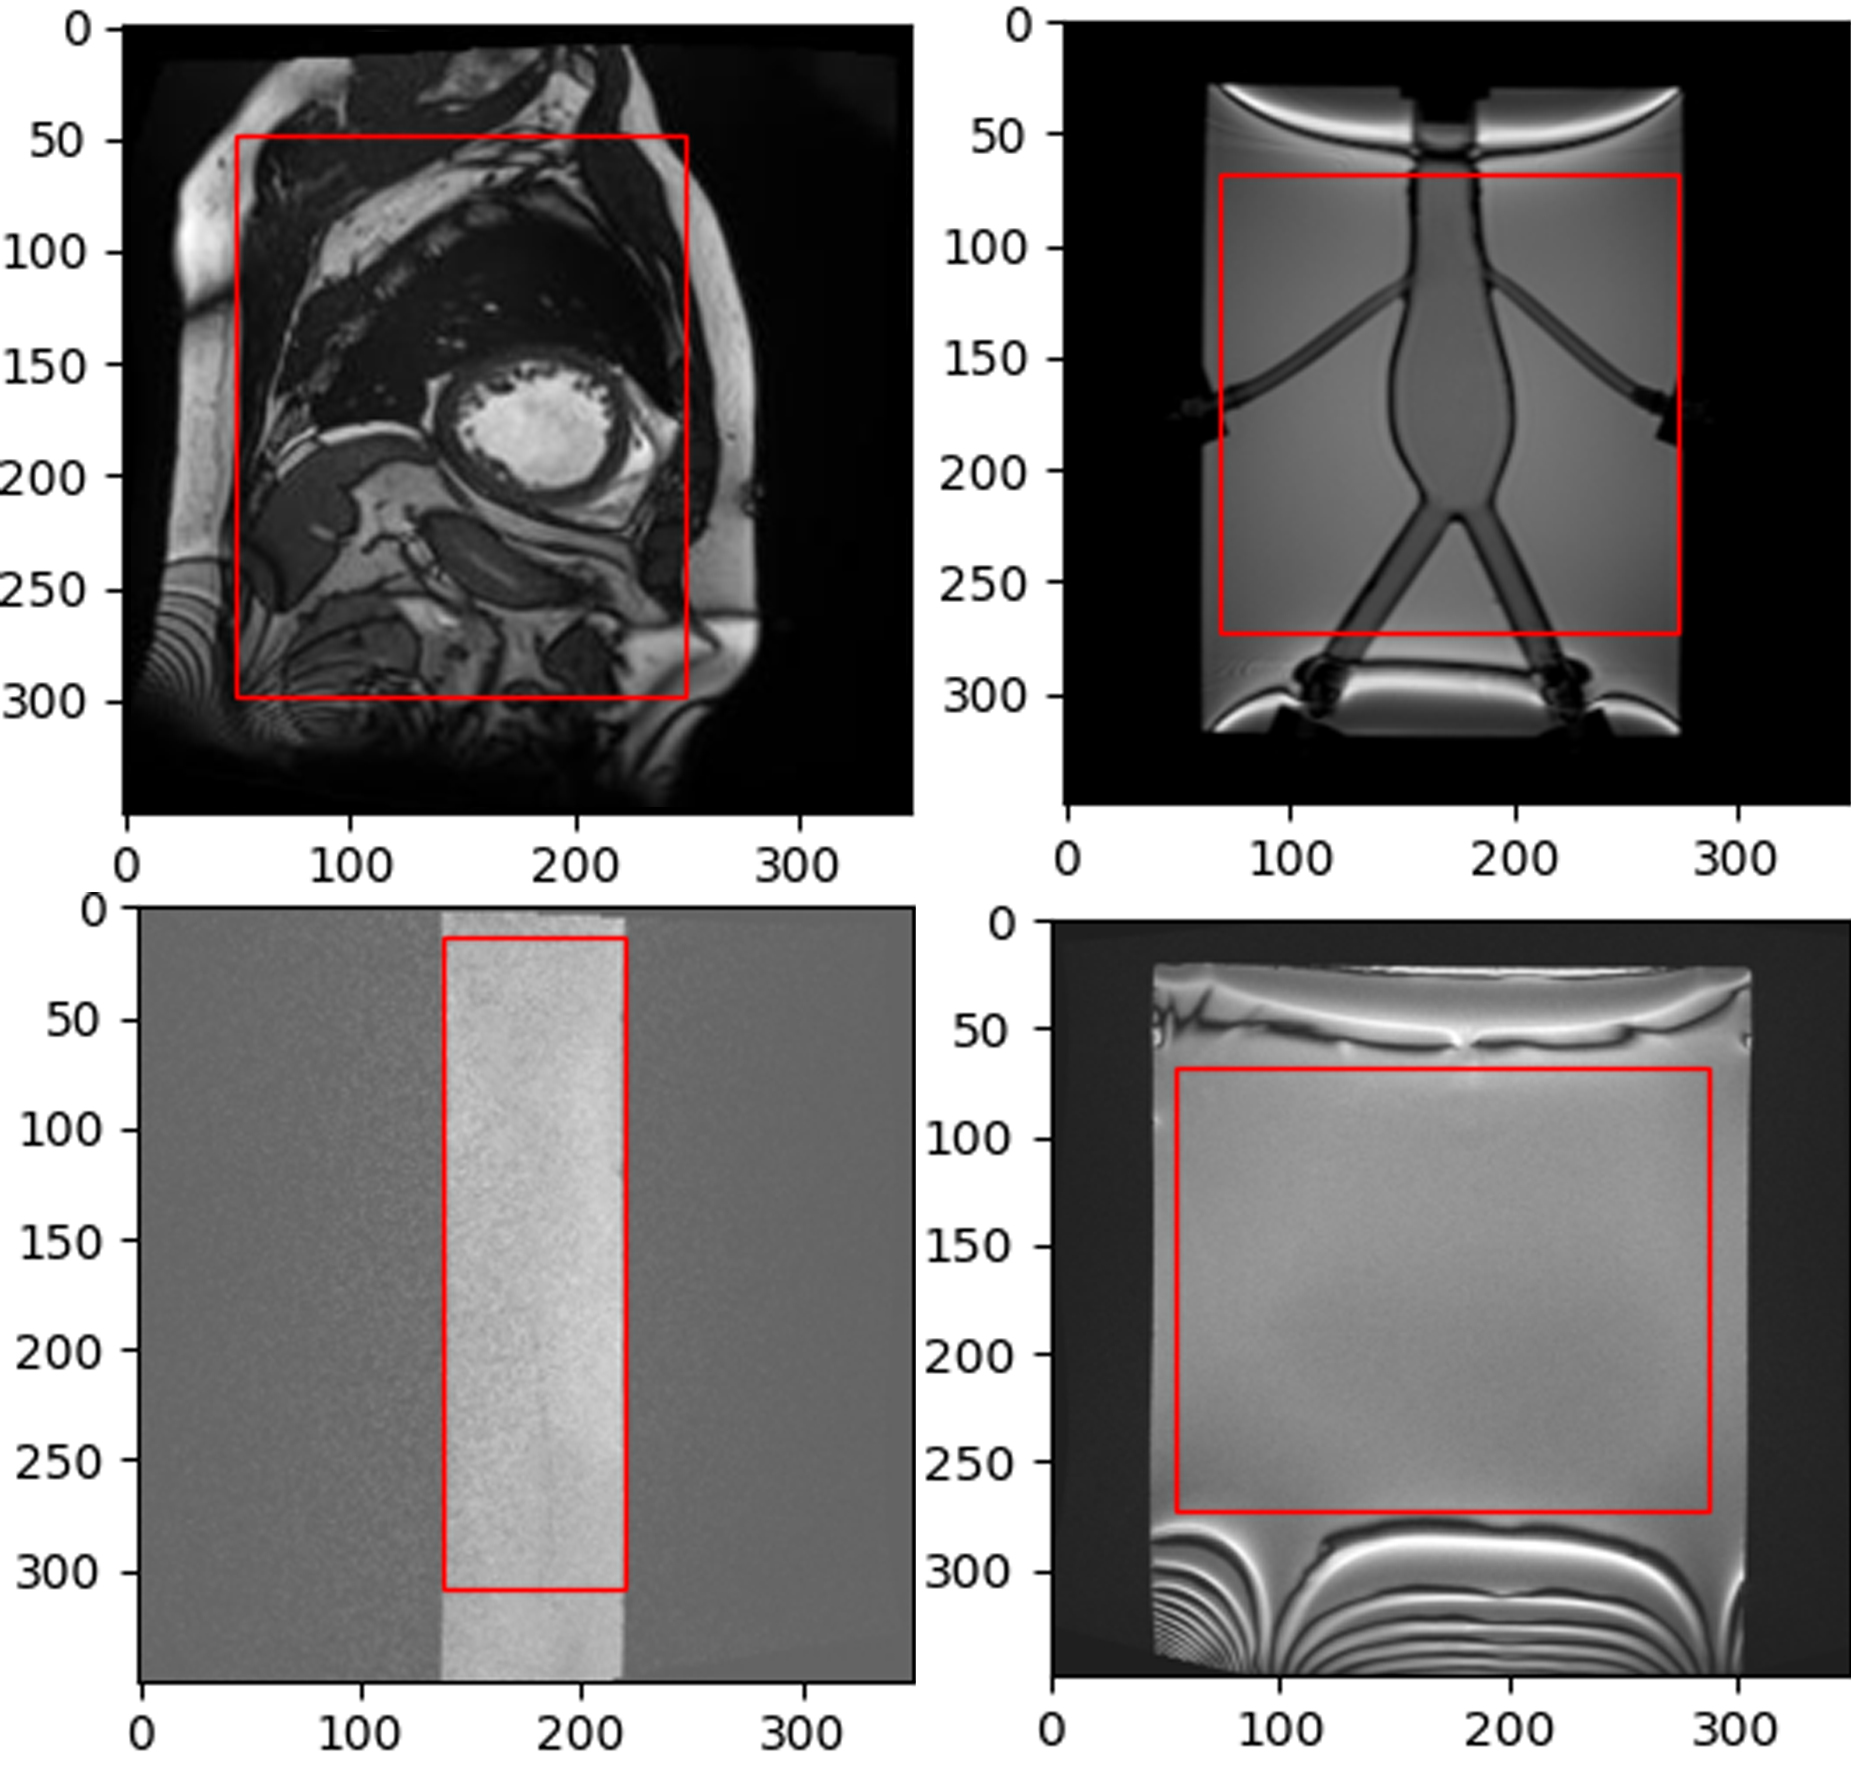
\includegraphics[width=1\linewidth]{Conference//img/roi-example-background-dataset.png}
    \caption{Examples of background images with a red rectangle deliniating the region where physics-based marker artefacts are synthetically introduced.}
    \label{fig:background-dataset}
\end{figure}

\begin{figure}[h]
    \centering
    \begin{minipage}{0.241\textwidth}
        \centering
        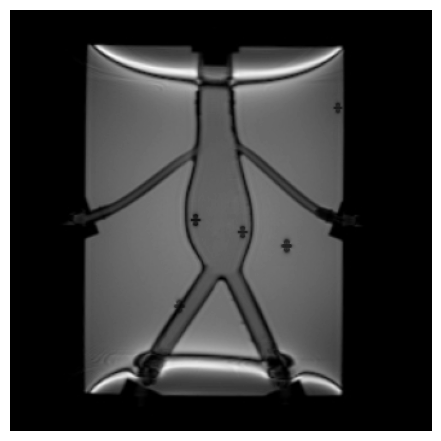
\includegraphics[width=\textwidth]{Conference/img/generated-image.png}
        \subcaption*{(a)}
    \end{minipage}\hfill \hspace*{0cm}
    \begin{minipage}{0.241\textwidth}
        \centering
        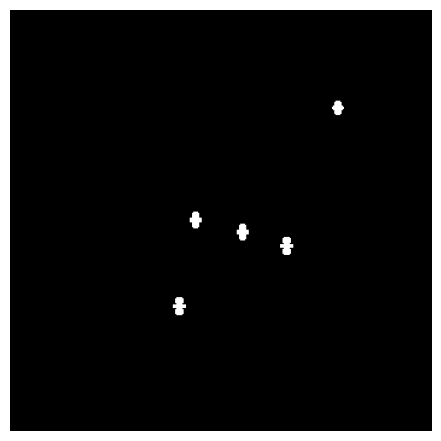
\includegraphics[width=\textwidth]{Conference/img/generated-image-truth.png}
        \subcaption*{(b)}
    \end{minipage}\hfill \hspace*{0cm}
    \caption{(a) Physics-based synthetically generated dataset image,
    (b) corresponding ground truth mask.}
    \label{fig:generated-dataset-and-truth}
\end{figure}

\subsection{Dynamic tracking}\label{guidewire-tracking}
In MRI-guided interventions, real-time tracking of the passive guidewire is essential for accurate device navigation, as well as automatic MRI slice movement to guidewire. However, there are many inherent challenges:
\begin{itemize}
    \item The guidewire can move out-of-plane;
    \item A low SNR can negatively impact detection performance;
    \item CNN can produce false positives;
    \item Flow artefacts and transient effects may impair the marker visibility.
\end{itemize}

To address these challenges, a dynamic tracking algorithm was developed, tailored to differentiate the movement of the guidewire from noise or false-positive CNN outputs. The tracking algorithm operates in conjunction with the CNN and can guide adjustments in the MRI imaging plane, to match the movement of guidewire. The algorithm takes the CNN output as input after applying a median filter to remove noise. This step removes the majority of false positives, which are usually small and localized in nature. The remaining outputs of the CNN are considered to be valid susceptibility artefacts and are continuously tracked by means of automated labeling. There could however still be false positives, as any paramagnetic inhomogeneity such as air or metal implants will create a susceptibility artefact similar to those produced by the guidewire \cite{pmid22162977}. However, those false positives are static in nature and stay in one position, as opposed to the guidewire which is in movement.

To differentiate the artefacts produced by the static background from those produced by the guidewire, an approach is used which combines euclidean distance-based matching with linear trajectory prediction. The algorithm maintains a list of tracked locations stored as trackers, each associated with a detected artefact. In each frame, each tracker location is updated based on the detected artefacts in that frame and the one preceding. When an artefact is not found within a specified euclidean distance for more than a predefined number of frames, it is considered lost and removed from the list of active trackers. This allows for smooth continuous tracking where some markers can temporarily disappear and re-appear, while removing false positives.

To estimate and predict the movement of guidewire, each tracker has a initial position and new position for each frame (demonstrated in \autoref{fig:tracking-algorithm} as large circles). The difference of each initial and updated position from the trackers is averaged, filtering small differences e.g. such as those induced by the static background. This results in an average displacement vector which represents the displacement of the guidewire. Based on the displacement vector, the imaging plane can be moved track the guidewire.

\section{Results}

\subsection{MRI sequence optimization}

A comparison and analysis in marker conspicuity for variations in slice thickness is shown for both the bSSFP and GRE sequences in \autoref{fig:MRI-sequence-optimization}. Overall, the bSSFP based images show to produce a higher SNR, and both sequences show an optimum marker CNR at a slice thickness of $d = 5$ mm, which corresponds to the approximate cross-section of the marker artefact. A larger slice thickness may be employed to reduce out-of-plane movement of the guidewire, at the cost of CNR. For imaging purposes, the optimal trade-off for slice thickness is around 10mm, as the CNR is still high and the extra thickness provides flexibility for guidewire movement.

\begin{figure}
    \centering
    \begin{minipage}{0.241\textwidth}
        \centering
        \includegraphics[width=\textwidth]{Conference/img/bssfp-CNR_new.png}
        \subcaption*{(a)}
    \end{minipage}\hfill \hspace*{0cm}
    \begin{minipage}{0.241\textwidth}
        \centering
        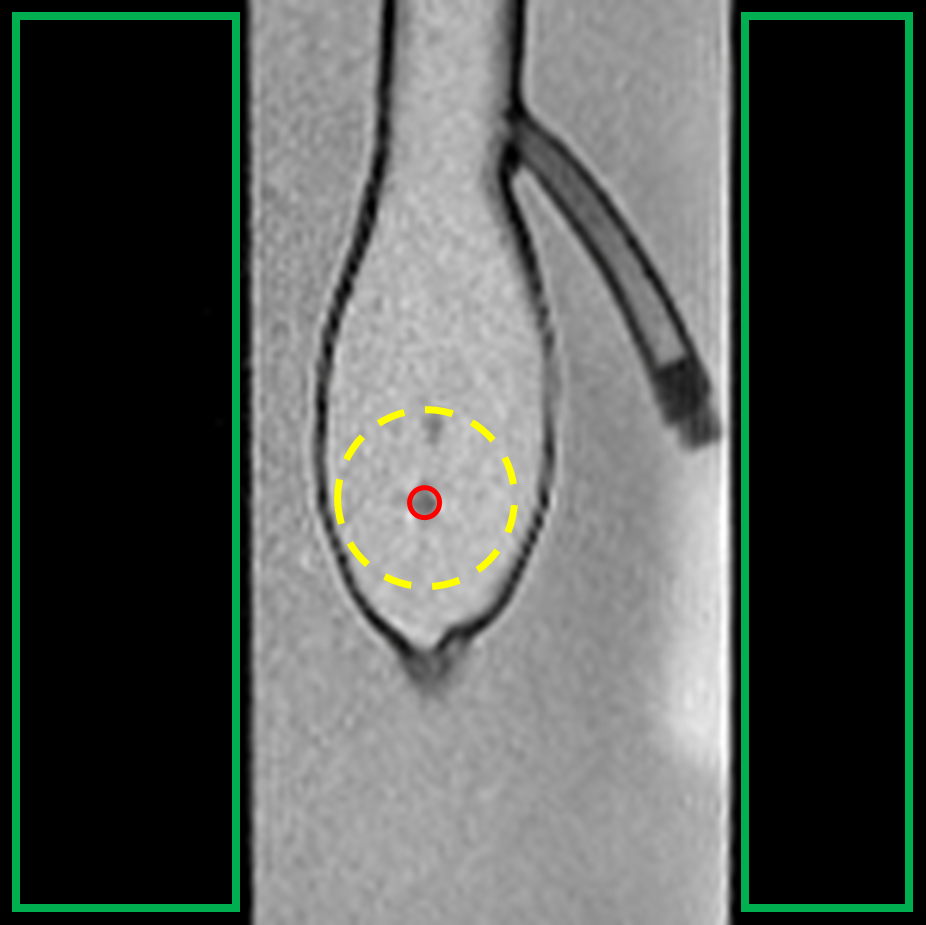
\includegraphics[width=\textwidth]{Conference/img/GRE-CNR_new.png}
        \subcaption*{(b)}
    \end{minipage}\hfill \hspace*{0cm}
    \begin{minipage}{0.48\textwidth}
        \centering
        \includegraphics[width=\textwidth]{Conference/img/CNR-comparison2.png}
        \subcaption*{(c)}
    \end{minipage}\hfill \hspace*{0cm}
    \caption{(a) Example sagittal bSSFP and (b) GRE images showing the noise ROI (green), lumen ROI (yellow) and marker ROI (red) used in contrast-to-noise (CNR) calculations. (c) Variation of marker CNR with slice thickness for both sequences.}
    \label{fig:MRI-sequence-optimization}
\end{figure}

\subsection{Susceptibility artefact model}

The parameters associated with the marker artefact were chosen to match those used experimentally, as listed in \autoref{table_MRI_parameters}. In the simulated model the field-of-view (FOV) was chosen smaller, which would later be scaled to match the actual artefact size. Additionally, the following parameters were used:
\begin{itemize} 
    \item \(B_0\): 1.5 T
    \item \(\Delta{\chi} V\): 0.012
    \item \(d\): 5-30 mm
\end{itemize}

Using these settings, the dipole field (\autoref{eq:dipole-field-distortion}) is calculated and integrated over the slice-thickness as defined in (\autoref{eq:integration-over-slice-formula}). A linear grayscale colormap is applied on the resulting field simulation, to get the output shown in \autoref{fig:simulations}. The superimposed simulations are compared with real artefacts in figure \autoref{fig:real-artefact-vs-simulated-comparison}.

\begin{figure}[h]
    \centering
    \begin{minipage}{0.241\textwidth}
        \centering
        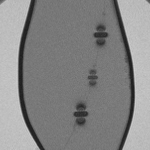
\includegraphics[width=\textwidth]{Conference/img/artifact-real.jpg}
        \subcaption*{(a)}
    \end{minipage}\hfill \hspace*{0cm}
    \begin{minipage}{0.241\textwidth}
        \centering
        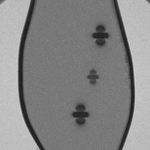
\includegraphics[width=\textwidth]{Conference/img/artifact-generated-superimposed.jpg}
        \subcaption*{(b)}
    \end{minipage}\hfill \hspace*{0cm}
    \caption{(a) True artefacts (b) synthetically generated artefacts.}
    \label{fig:real-artefact-vs-simulated-comparison}
\end{figure}

\subsection{CNN training}

Using the procedural dataset generation described in \ref{artefact-cnn-dataset}, approximately 1000 images were generated to train the CNN.

Using the nnUNet architecture, a standard of five cross-validation folds was performed during training, where the best performing fold was selected for inference and real-time prediction. The dataset was randomized and split to $80/20$ \% during training and validation, respectively, at the end of each fold. The CNN was trained until approximate convergence at 100 epoch. The training achieved a pseudo-DICE score of 0.9957 and best Mean Validation Dice of 0.9974.

Accuracy and latency during real-time inference can be described as sufficient. The real-time inference latency for the prediction was around 0.3 seconds on a NVIDIA RTX 3090 GPU. This time significantly increased when using slower GPUs. Most of the time, all visible non-distorted artefacts were detected. During rapid guidewire movement, disturbance caused by transient effects resulted in some detection gaps for 1-2 frames (\autoref{fig:flow-artefacts-tracking}). False positives that can not be filtered out (e.g. fixation screws discussed in \ref{guidewire-tracking}) were to be expected and were also detected by the CNN.

\subsection{Dynamic tracking performance}

Tracking slow guidewire movement was stable and accurate. As the guidewire speed increases, the transient effects become increasingly destructive, causing the tracking to lose context and re-initialize once the guidewire has slowed down enough. An example of transient effects is shown in \autoref{fig:flow-artefacts-tracking}.

Tracking itself can not easily be quantified, as the accuracy is heavily dependent of the CNN. The center coordinates of each tracker is chosen to be the centroid of the detected artefact. That means, due to the slight inconsistencies of the CNN, the center coordinates can vary within the confines of the detected artefact, translating to ~$\pm$5 mm of possible fluctuation in artefact position in MRI reference axis. The fluctuation typically only applies to instable detections in areas of low SNR. Slice alignment accuracy is likely higher, as all trackers are considered for calculating the displacement vector.

\begin{figure}[ht]
    \centering
    \begin{minipage}[t]{0.49\textwidth}
        \centering
        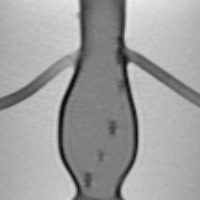
\includegraphics[width=0.49\linewidth]{Conference/img/tracking-websocket-start.jpg}
        \vspace{0.1cm}
        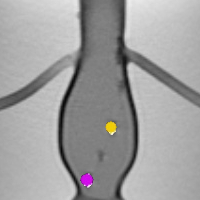
\includegraphics[width=0.49\linewidth]{Conference/img/tracking-websocket-tracks-start.jpg}
    \end{minipage}
    \begin{minipage}[t]{0.49\textwidth}
        \centering
        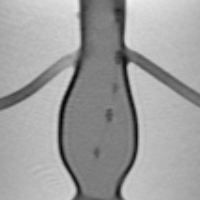
\includegraphics[width=0.49\linewidth]{Conference/img/tracking-websocket-end.jpg}
        \vspace{0.1cm}      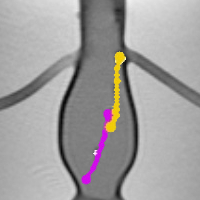
\includegraphics[width=0.49\linewidth]{Conference/img/tracking-websocket-tracks-end.jpg}
    \end{minipage}
    \caption{Guidewire tracking progress. Limited to 2 trackers for visualization purposes, 2-3 markers detected using CNN.}
    \label{fig:tracking-algorithm}
\end{figure}

\begin{figure}[ht]
    \centering
    \begin{minipage}{0.241\textwidth}
        \centering
        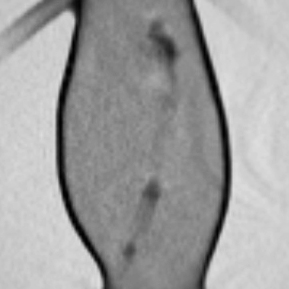
\includegraphics[width=\textwidth]{Conference/img/flow-artifact-with.jpg}
        \subcaption*{(a)}
    \end{minipage}\hfill \hspace*{0cm}
    \begin{minipage}{0.241\textwidth}
        \centering
        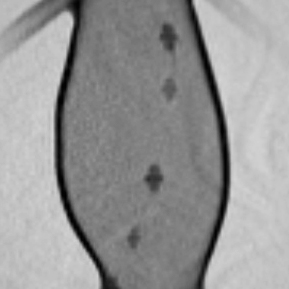
\includegraphics[width=\textwidth]{Conference/img/flow-artifact-without.jpg}
        \subcaption*{(b)}
    \end{minipage}\hfill \hspace*{0cm}
    \caption{(a) Transient effects when moving guidewire very fast
    (b) Image after re-establishing steady state magnetization after movement}
    \label{fig:flow-artefacts-tracking}
\end{figure}


\section{Discussion and Conclusion}

\subsection{Summary of findings}
Our physics-based approach to susceptibility artefact simulation showed to be both accurate and flexible, allowing the generation of large amounts of training data. Although the accuracy of the model might be further improved by implementing more specific signal descriptions for bSSFP as discussed in \cite{sunil-patil-phd}, the current simulation was observed to be sufficient as the susceptibility artefacts due to the relatively low spatial resolution used.

Using the physics-based dataset can be considered very effective as it saved the effort of manually annotating and acquiring images experimentally. It also provides flexibility to train the CNN on existing datasets, or even subject-specific data. Due to the unique and predictable shape of the susceptibility artefact, the training was able to achieve a very high mean and DICE accuracy. This accuracy also translated into accurate real-time detection.

The detection performance of the CNN could be further improved for specific circumstances, e.g. transient effects and noisy images. Under controlled conditions such as the current phantom, the detection was good and once any noise was filtered out it was nearly perfect. Further testing is required to evaluate the detection accuracy in in-vivo situations. It may be expected to drop as the surrounding anatomy will make detection harder due to lack of contrast between the background and the marker artefact.

Despite the ad-hoc nature of our tracking algorithm a smooth performance was observed under the test scenarios. Optimal tracking performance relies on the accuracy of the CNN and was found to work well under the situations explored. The algorithm was also found to be robust against cases where the guidewire approaches the edge of the lumen, leading to artefact temporarily disappearing. The dynamic tracking performance appeared to be most affected when the CNN detection performance is poor, for instance when using a very low SNR image.

\subsection{Results comparison}
Han Nijsink et al. used manual annotation for marker locations from a training dataset of 30 images, with 10 images for validation \cite{pmid35199259}. They achieved similar results, where median number of markers detected from images was equal to the amount of markers in the images. They suggested the use of GRE sequences instead of bSSFP as used here, as GRE does not have passive banding artefacts and is less prone to flow artefacts and transient effects. However during our testing, GRE sequences could not achieve the same real-time performance as bSSFP. The SNR for bSSFP sequence with a repetition time of 0.5 seconds was significantly better than GRE. In the end, the ability to synthetically generate the training dataset allows for adapting the sequence and retraining the CNN very efficiently.

\subsection{Future work and current limitations}

The project has not addressed the safety aspect of MR interventions yet. Safety could be improved by additional visualizations, for instance showing where the guidewire might be colliding with a vessel wall. This would require keeping track of the guidewire's movement in three-dimensions, as well as basic anatomy detection, such as 3D mapping vessels.

As the complete software system relies heavily on the CNN, improvements and stabilizing the detection even further would be beneficial. The current system is trained mostly for phantom-based images, a small subset of training data includes anatomical data, and inference on anatomical data has not been concluded. Considering the background anatomy could open up possibilities for in-vivo detection. Additionally, the detection currently only considers susceptibility artefacts which are parallel with the $B_0$ orientation. Oblique detection is not considered but could be beneficial. Furthermore, heatmap regression approaches could be considered such as those used in anatomical landmark detection.

The current tracking algorithm is limited to changing MRI slice in only 2 axis MRI X and Z). Moving in Y direction requires development of a three-dimensional tracking algorithm, which could understand if guidewire is going upwards or downwards from the slice. 

\subsection{Conclusion}
Our proof-of-concept study has shown the potential of an automated passive tracking approach in the context of endovascular interventions. The proposed technique is able to detect susceptibility artefacts and dynamically track a guidewire using real-time MRI sequences, eliminating need for manual slice alignment. By optimizing the guidewire visibility, a robust detection performance of the approach was observed, while still being responsive enough for real-time feedback. This may provide a cost-effective solution to improve MR-guided interventions.

% \section*{Acknowledgment}
\bibliographystyle{vancouver}
\bibliography{references}
\vspace{12pt}

\end{document}
